%************************************************
\chapter{Hidden Markov Random fields for biological data clustering}\label{ch:HMRF} 
%************************************************
This Chapter gives a theoretical overview of a Hidden Markov Random Field based approach that is designed to cluster single cell in-situ hybridization gene expression data ``cubes'' as described in Chapter \ref{ch:singlecell}, into $K$ clusters ($K \in {2, 3,...}$). Subsequently, we will describe our approach for estimating $K$.

	\section{background}
	Markov random fields (MRF) are statistical models that provide a way of modeling entities composed of multiple discrete sites such as images where each site is a pixel or in our case a biological tissue where each site is a single cell, in a context-dependent way \citep{li09}. MRF based methods find their roots in the field of statistical mechanics as the Ising model \citep{Ising25} and its generalization, the Potts model \citep{Wu82}. Since then, they have been and are still mainly used in the field of image analysis, and the literature about them is ever growing \citep{rozanov82,li95}. More specifically MRF methods are found in a wide range of applications such as image restoration and segmentation \citep{zhang01}, surface reconstruction \citep{paulsen10}, edge detection \citep{zerubia93}, texture analysis \citep{clausi04}, optical flow \citep{heitz93}, active contours \citep{martin05}, deformable templates \citep{mignotte01}, data fusion \citep{wright89} and perceptual grouping \citep{fields97}.\\
	
	MRF have also been used in a variety of biological applications from analysing medical imaging data \citep{zhang01,held97,descombes98} to analysing networks of genomic data \citep{wei07}. In the context of the shift from the tissue to the single cell scale in transcriptomics assays described in the previous chapters, MRF based method represent a natural way to model gene expression in single cells while accounting for the relationship between sites.\\
	
	 Mathematically, MRF models are built around two complementary sub-models. On the one hand, the field represents the sites and their spatial structure central to the MRF theory. It is given a mathematically sound form through the Hammersley-Clifford (1971) theorem which sates that the influence between sites in a field following the Markov properties follows a Gibbs distribution dependent upon an Energy function in which the spatial coherency parameters of the model are incorporated. This theorem gives strong mathematical bases for modeling spatially dependent data. In this part of the model, some essential technical choices have to be made namely the \emph{neighbourhood system} and the \emph{Energy function} used. On the other hand, the emission model represents the data and the observations, introducing a certain number of parameters depending on the type of data modeled.\\
	 
	 In the next paragraphs I will present the technical choices made to apply this mathematical framework to the single cell in-situ hybridization dataset of \platy{}'s brain. I will also present the implementation of a EM algorithm used to find the maximum a posteriori (MAP) estimates of the model's parameters, classifying this method into the MAP-MRF framework.

\section{Markov random fields}
	

	\subsection{Neighbourhood systems}\label{sec:neighbours}
Let $S$ be a finite set of sites, each of which represents one ``cube'' of data. Given the 3D coordinates of each site, the first challenge that needs to be overcome in order to use the spatial characteristics of the data in the clustering scheme is to express the data and their spatial relationship in a mathematically formal manner. To this end, starting from the spatial coordinates in 3D of each ``cube'', instead of a list of isolated measurements, it is possible to build a connecting graph representing the same data and the spatial dependence between the ``cubes''. In the context of this study, each node of the graph will represent a ``cube'' in the single cell expression data. Nodes that are linked together by an edge will be spatially dependent upon each other.\\

With prior biological data, one can manually create the spatial dependency graph by linking nodes together that are known to be functionally similar. In the case of this study, however, no such prior knowledge being available, it is necessary to define the spatial dependences in a different way.\\

The central hypothesis while developing this method is to assume that ``cubes'' that are close to one another are more likely to belong to the same cell type (i.e cluster). Consequently, these spatial dependencies will be incorporated into a \emph{neighbourhood graph} where  ``cubes'' close to each other will be joined.\\

In the case of this study, because of the cell model used the graph will be a regular grid. In this context, there are several ways to translate the spatial relationship into neighbourhood graphs depending upon the number of neighbours considered for each site. As shown in Figure \ref{fig:graph}, the choice between a first or a second order neighbourhood system is purely technical. However, having more neighbours for each site will increase the complexity and ultimately the computational burden. Within $G$, a \emph{clique} $c$ is a subset of nodes that are all interconnected, i.e it is possible to go from any nodes in $c$ to any other node in $c$ by simply following one single edge.\\

	\begin{figure}[H]
\centerline{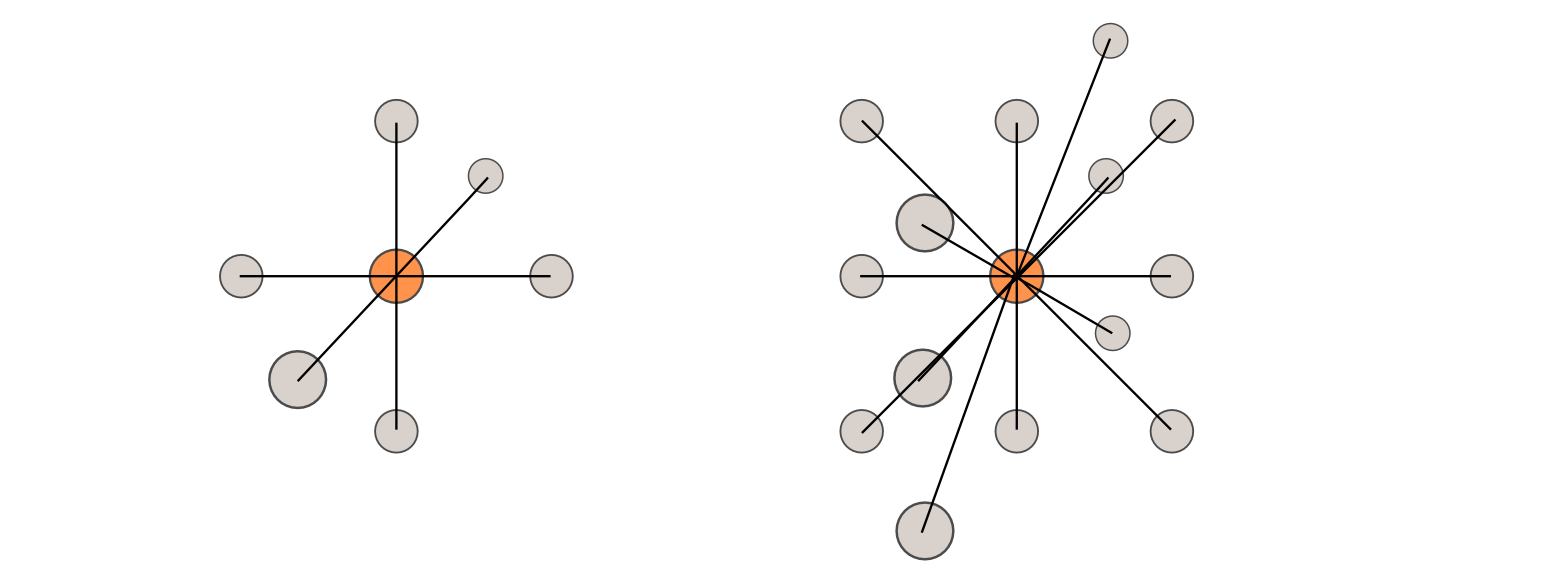
\includegraphics[width=0.8\linewidth]{gfx/chapter4/graph.png}}
\caption{{\bf First order and second order neighbourhood systems.} In the first order neighbourhood system, each site in the graph is linked to a maximum of 6 other sites in 3D while in the second order neighbourhood system each site can be linked to a maximum of 14 other sites. The Markov property on the graph implies that the state of any node (the orange one for example) can be fully determined by knowing the state of its neighbours (the grey ones).}\label{fig:graph}
	\end{figure}

	Let $C$ be the set of cliques of $G$. In a first order neighbourhood system, $C$ is therefore the set of all sites alone and all the pairs of sites that are neighbours of one another. These are first and second order cliques, containing one or two sites. In a second order neighbourhood graph however, the set of all cliques in $G$ also contains 3rd and 4th order cliques. Because the method implies iterating over the set of all cliques of the graph as I will detail in the next paragraphs, I decided to use a first order neighbourhood system to decrease the computational burden.


	\subsection{Field distribution}
Let a Random Field $Z$ be defined as a set of random variables $Z = \{Z_i , \forall i \in S\}$ where $Z_i \in {1,...,K}$. For every site $i \in S$, let $N(i)$ represent the set of its neighbours (see \ref{sec:neighbours}) and $\boldsymbol{z_{S-\{i\}}}$ a realization of the field restricted to $S-\{i\} = \{j \in S, j \neq i\}$. $Z$ is a \emph{Markov Random Field} if and only if it follows the Markov property at every site :

\begin{align}
\label{eq:markov1}
\forall i \in S, P_G (z_i \mid z_{S-\{i\}}) = P_G (z_i \mid z_j , j \in N(i))
\end{align}

Equation (\ref{eq:markov1}) states that the realization of the field, $z_{i}$ at any site $i \in S$ can be fully determined using only the state of its neighbours $N(i)$. In other words the probability that a ``cube'' is in a given state depends only upon the state of its neighbours.\\

The Hammersley-Clifford theorem states that if $Z$ is a Markov Random Field, the joint distribution of the field $P_G$ follows a Gibbs distribution such that :

\begin{align}
\label{eq:prior}
P_G (\boldsymbol{z;\beta}) &= W(\boldsymbol{\beta})^{-1} \exp{(-H(\boldsymbol{z;\beta}))} \nonumber\\
&= \frac{e^{-H(\boldsymbol{z;\beta})}}{\sum\limits_{\boldsymbol{z'}} e^{-H(\boldsymbol{z;\beta})}}
\end{align}

with $H(\boldsymbol{z})$ the Energy function summed over the cliques $C$ of the graph $G$. Since we are working with a first order neighbourhood system, $C$ is the set of all pairs of sites $(i,j)$ that are neighbours. We chose to consider $H$ as a function of a vector $\boldsymbol{\beta} = (\beta_1, \hdots, \beta_K)$ containing $K$ parameters as detailed in the next paragraph, and $v_{i,j}$ a potential function set to 1 in our method because we are working on a regular grid graph. If the distances between sites were heterogeneous we could have used this function to weight the spatial dependence between sites. Given this set up, we can write

\begin{align}
\label{eq:Energy}
H(\boldsymbol{z}) = - \sum\limits_{i \in S}\beta_{z_i}\sum_{\substack{j \in N(i)}}v_{i,j}\times\boldsymbol{1}_{[z_i = z_j]} 
\end{align}

The denominator in (\ref{eq:prior}), where $\boldsymbol{z'}$ represents all the possible realizations of the field, is a normalizing constant referred to as $W(\boldsymbol{\beta})$.\\

	\subsection{Single and multiple beta models in a biological context}
This model is closely related to a K-colour Potts model \citep{Wu82}. However, the unusual nature of the data used in this thesis led to the idea of extending the model commonly used in the field of image segmentation. In particular, the K-colour Potts model defines a single spatial coherency parameter $\beta$ that is shared by all clusters \citep{subudhi14,zhang14}. Importantly, the method presented here was extended by assigning one $\beta$ per cluster so that:
\begin{equation*}
\label{eq:beta}
\boldsymbol{\beta} = (\beta_{1},...,\beta_{K})
\end{equation*}

 Interestingly, equation (\ref{eq:Energy}) is a decreasing function of every component of $\boldsymbol{\beta}$. Indeed, for a particular cluster $h \in K$, a high value of $\beta_h$ will accentuate the increase of the likelihood of the model through equation (\ref{eq:prior}) when cluster $h$ is spatially coherent. In other words, when a site has all its neighbours clustered in cluster $h$, classifying the site in cluster $h$ (making cluster $h$ spatially more coherent) will have an impact on the likelihood of the model proportional to the value of $\beta_h$. This Energy function thus favours spatially regular partitions and a higher value of $\beta_h$, with $1 \leq h \leq K $ will amplify the smoothing effect, or coherence over cluster $h$.\\
 
 The choice of an extended model with a multiple $\boldsymbol{\beta}$ parameter, is inherent to the data used in this thesis. The first motivation is purely cytological: In a biological context, it is expected that some tissues will be more spatially coherent than others. As mentioned in the Introduction and visualized in Figure \ref{fig:cells}, tissues composed of different cell types may interact differently with their neighbours. For example, differentiated neural cells with long axons are likely to be in contact with numerous other cell types that they pass through.\\
 
  The second motivation for the extended model lies in the cell model described in \ref{sec:single_cell_insitu}. As described in Figure \ref{fig:cubeserrors}, some ``cubes'' may have inconsistent gene expression patterns. This type of error in the data will introduce spatial incoherence in the gene expression patterns. I also mentioned in Chapter \ref{ch:singlecell} that the rate of errors linked to the experimental protocol may be dependent upon the cell type considered. Indeed, the errors described in Figure \ref{fig:cubeserrors} are respectively more likely to arise in cell types with small and big cells. In summary, I believe that allowing one spatial parameter for each cluster enables a better smoothing of these potential experimental errors by accounting for cell type specificity.\\
 
 \subsection{Field parameters}

The field distribution contains $K$ unknown parameters $\boldsymbol{\beta} = (\beta_{1},...,\beta_{K})$ that have to be estimated by the model. It is important to note that $W(\boldsymbol{\beta})$ is summed over all possible realizations of the field $Z$, which is an exponentially complex sum as the cardinality of $S$ rises. Therefore the computation of the normalizing factor becomes intractable very quickly. To address this problem, we are going to need to make some approximations in order to compute this quantity (see Mean Field Approximations).\\

\section{The emission model}

We have described the field distribution of a Markov Random Field representing our graph, we now need to describe the relationship between $Z$ and the data.

\subsection{Conditional independence in the observed data}
As $Z$ is unknown a priori and represents the partition, let $Y$ be a set of random variables representing the observations (the in-situ hybridization data). The model requires a conditional independence assumption with regard to the observations $Y$ given the partition $Z$ so that, with $f_{z_i}$ the density function relative to cluster $z_i, i \in S$ (the realization of the field at node $i$):

\begin{align}
p(\boldsymbol{y} \mid \boldsymbol{z} ; \Theta) &= \prod_{i \in S} p(y_i \mid z_i ; \Theta) \nonumber\\
\label{eq:independence}
&= \prod_{i \in S} f_{z_i} (y_i \mid z_i ; \Theta)
\end{align}

Equation \ref{eq:independence} defines one unknown parameter per cluster: $\Theta = (\boldsymbol{\theta_1},...,\boldsymbol{\theta_K})$. It is interesting to note that this part of the model is equivalent to an independent mixture model \citep{mclachlan04}. Indeed, Markov random fields can be viewed as independent mixture models where $Z$ is a set of independent, identically distributed random variables, which happens when $\beta = 0$.\\

Given a particular cluster $h \in {1,...,K}$ and M the set of considered genes, the expression of each gene $m \in M$ in cluster $h$ is modelled by a Bernoulli distribution with parameter $\theta_{h,m}$. This leads to one unknown Bernoulli parameter per gene per cluster so that :

\begin{align*}
\Theta &= (\boldsymbol{\theta_1},...,\boldsymbol{\theta_K})\\
&= \left( \begin{array} {ccc}
\theta_{1,1} & \ldots  & \theta_{1,_K}\\
\vdots & \ddots & \vdots\\
\theta_{M,1} & \ldots & \theta_{M,_K} \end{array} \right)
\end{align*}

	\subsection{Full likelihood of the Hidden Markov random field model}

The conditional density function $f_i, i \in S$ can be expressed as :

\begin{align}
f_i(y_i \mid z_i ; \Theta) &= f_i(y_i \mid z_i ; \boldsymbol{\theta_{z_i}}) \nonumber\\ 
&= \prod_{m \in M} \theta_{z_i,m}^{y_{i,m}} \times (1-\theta_{z_i,m}^{1-y_{i,m}})
\end{align}

Looking at both fields $Z$ and $Y, Z$ together, the complete likelihood of the model is expressed as :

\begin{align}
\label{eq:likelihood}
P_G(\boldsymbol{y},\boldsymbol{z} \mid \Theta, \boldsymbol{\beta}) &= f(\boldsymbol{y} \mid \boldsymbol{z}, \Theta)P_G(\boldsymbol{z} \mid \boldsymbol{\beta})\nonumber\\
&= W(\boldsymbol{\beta})^{-1}exp\{{-H(\boldsymbol{z} \mid \boldsymbol{\beta})} + \sum\limits_{i \in S}log(f_i(y_i \mid z_i, \theta_{zi}))\}
\end{align}

Because equation (\ref{eq:likelihood}) is a Gibbs distribution, using the Hammersley-Clifford theorem we can conclude that the conditional field $Z, Y$ is another Markov Random Field with the Energy function 
\[H(\boldsymbol{z}, \boldsymbol{y} \mid \boldsymbol{\beta}, \Theta) = H(\boldsymbol{z} \mid \boldsymbol{\beta}) - \sum\limits_{i \in S} log(f_i(y_i \mid z_i, \Theta))\]

In our case, the goal is to recover the unknown realization of $Z: \boldsymbol{z}$. To this end we need to maximize the values of all the parameters of the model $\boldsymbol{\psi} = (\boldsymbol{\Theta}, \boldsymbol{\beta})$, and to chose the optimal number of clusters, $K$.

\section{Parameter estimation using the EM algorithm}
As mentioned before, the aim is to assign each cell $i$ to one of the $K$ possible clusters. To do so, it is interesting to consider the Maximum Posterior Marginal (MPM) that maximizes $P(Z_{i}=h|\boldsymbol{y}, \boldsymbol{\psi})$, where the $\boldsymbol{\psi}$ are unknown and need to be estimated. To this end, the Expectation Maximisation \citep{dempster77} (EM) principle can be applied. The EM algorithm consists in the Expectation step (E) where the expectation of the model's likelihood with the current parameters is computed and the Maximization step (M) where the latent variables that maximize the model's expectation computed in the E step are found. The two steps are repeated until a convergence factor is reached.\\

	\subsection{Initialization}
The first step of the algorithm is to initialize the model's parameter. To this end, it is possible to directly assign values for $\boldsymbol{\psi}^{0}$, or to generate an initial clustering $\boldsymbol{z}^{0}$ from which the initial $\boldsymbol{\psi}^{0}$ will be derived.\\

I decided to use a combination of both approaches, with arbitrary values assigned to $\boldsymbol{\beta}^{0}$, typically $0$, and the use of an initial clustering to compute the values of $\boldsymbol{\Theta}^{0}$. Indeed, for $h \in {1,...,K}, m \in M$, because of the emission model, each $\theta_{h,m}$ is the probability that $m$ is expressed in cluster $h$. Consequently, given a clustering $\boldsymbol{z}^{0}$ with function $Expr_{h,m}$ the number of cells expressing gene $m$ in cluster $h$ and function $Num_h$ the total number of cells in cluster $h$ I set:

\begin{align*}
\theta_{m,h}^{0} = \frac{Expr_{h,m}}{Num_h}
\end{align*}

	\subsection{E step}

In the E step the parameters are fixed and the expectation of the model's likelihood $Q(\boldsymbol{\psi} \mid \boldsymbol{\psi}^{l})$ at iteration $l > 0$ can be derived from equation \ref{eq:likelihood} as:

\begin{align}
Q(\boldsymbol{\psi} \mid \boldsymbol{\psi}^{l}) &= \sum\limits_{\boldsymbol{z}} p(\boldsymbol{z} \mid \boldsymbol{y} ; \boldsymbol{\psi}^{l}) log\:p(\boldsymbol{y},\boldsymbol{z};\boldsymbol{\psi}) \nonumber
\end{align}
Which can be further decomposed as :
\begin{align}
\label{eq:decomposed}
Q(\boldsymbol{\psi} \mid \boldsymbol{\psi}^{l}) &= \underbrace{\sum\limits_{\boldsymbol{z}} p(\boldsymbol{z} \mid \boldsymbol{y} ; \boldsymbol{\psi}^{l}) log\:p(\boldsymbol{y} \mid \boldsymbol{z} ; \Theta)}_{R_y(\Theta\mid \boldsymbol{\psi}^l)} 
 + \underbrace{\sum\limits_{\boldsymbol{z}} p(\boldsymbol{z} \mid \boldsymbol{y} ; \boldsymbol{\psi}^{l}) log\:p(\boldsymbol{z} \mid \boldsymbol{\beta})}_{R_z(\boldsymbol{\beta}\mid \boldsymbol{\psi}^l)}
\end{align}

Equation (\ref{eq:decomposed}) allows me to separately optimise $R_y$ and $R_z$.


$R_y$ can be re-written using equation(\ref{eq:independence}) as:

\begin{align*}
R_y(\Theta\mid \boldsymbol{\psi}^l) &= \sum\limits_{\boldsymbol{z}} p(\boldsymbol{z}\mid \boldsymbol{y} ; \boldsymbol{\psi}^{l})\;\sum\limits_{i \in S}\: log\: f_{z_i} (y_i ; \Theta)\\
&= \sum\limits_{i \in S} \sum\limits_{h=1}^{K}\; \left[log\: f_{h} (y_i  ; \Theta) \right] \; p(Z_i = h \mid \boldsymbol{y};\boldsymbol{\psi}^{l})
\end{align*}  

Therefore, in the M step I will need to compute the following probability:

\begin{align*}
t_{i\,h}^{l+1} = p(Z_i = h \mid \boldsymbol{y};\boldsymbol{\psi}^{l})
\end{align*}

Computing this conditional probability is problematic because of the dependence between neighbouring ``cubes'', and computing an exact value is computationally expensive. Indeed, each point being dependent upon its neighbours, and the neighbours being themselves dependent upon their neighbours, unsurprisingly computing these conditional probabilities becomes exponentially complex as the number of connected nodes in the graph grow. Additionally for $R_z$, as mentioned previously, it is also necessary to compute the value of the normalizing constant $W(\boldsymbol{\beta})$.\\

To compute those quantities, approximations are needed. Methods to do so include Besag's pseudo-likelihood \citep{Besag75} to compute $W(\boldsymbol{\beta})$, and simulating the posterior distribution of $Z$ given $\boldsymbol{y}$ with the parameters at iteration $l$, with a Gibbs sampler to estimate $t_{i\,h}^{l+1}$ \citep{Chalmond89}.\\

However, another method exists, the mean field approximation originally proposed in the field of statistical mechanics. Since then, it has been used in a variety of fields including computer vision \citep{Yuille90} and more recently to approximate the distribution of both $W(\boldsymbol{\beta})$ (with a single $\beta$) and $t_{i\,h}^{l+1}$ \citep{Zhang92}. I present here the extension of this method to a model with one $\beta$ parameter per cluster.

\section{Mean field approximations}

The idea behind this approximation is to compute intractable quantities at any point $i \in S$ by setting all the other sites in the field to their mean values. Keeping in mind the Markov property expressed in equation (\ref{eq:markov1}), when considering a single site $i \in S$, setting all the other sites in the graph to a defined value is equivalent, in the case of an MRF, to setting only the values of $N(i)$.\\

When computing $t_{i\,h}^{l+1}$, the mean fields approximation yields the following fixed point equation for $i \in S$ and $1 \leq h \leq K$ \citep{Dang98}:

\begin{align}
\label{eq:fixedpoint}
t_{i\,h}^{l+1} \approx \frac{f_{h} (y_i;\boldsymbol{\theta}_{h}^l)\; exp\{\beta_h^l \: \sum_{j \in N(i)} t_{j\,h}^{l+1}\}}{\sum_{u=1}^K \: f_{u} (y_i;\boldsymbol{\theta}_{u}^l)\; exp\{\beta_u^l \: \sum_{j \in N(i)} t_{j\,u}^{l+1}\}}
\end{align}


For the normalizing constant $W(\boldsymbol{\beta})$, by applying the mean-field approximation, using equation (\ref{eq:Energy}), $W(\boldsymbol{\beta})$ can be written as:

\begin{align*}
W(\boldsymbol{\beta}) = \sum\limits_{\boldsymbol{z'}} exp(-H(\boldsymbol{z'})) \approx \sum\limits_{i \in S}\;\sum\limits_{\boldsymbol{z_i}} exp(-H(\boldsymbol{z_i})) = \sum\limits_{i \in S}\;\sum\limits_{\boldsymbol{z_i}} exp(\beta_{z_i}\sum\limits_{j \in N(i)}1[z_i=z_j])
\end{align*}

With this new set of equations, it becomes possible to estimate all quantities needed in the E step in order to compute the model's expectation.\\

\section{M step}
After the E step, maximizing $\boldsymbol{\psi}$ is relatively straightforward. Equation \ref{eq:decomposed} yields:

\begin{align*}
\Theta^{l+1} &= arg\:\underset{\Theta}{max}\:R_y(\Theta\mid \boldsymbol{\psi}^l)\\
\boldsymbol{\beta}^{l+1} &= arg\:\underset{\boldsymbol{\beta}}{max}\:R_z(\boldsymbol{\beta}\mid \boldsymbol{\psi}^l)
\end{align*}

For $\Theta$, once the the $t_{i\,h}^{l} = p(Z_i = h \mid \boldsymbol{y};\boldsymbol{\psi}^{l})$ have been computed during the E-step, those probabilities may be used to assign each cell to its most probable cluster at step $l$. This is as hard clustering approach, which is a technical choice but of course the probabilities $t_{i\,h}^{l}$ could instead be used to compute a fuzzy clustering criterion for instance, the Hathaway's fuzzy clustering criterion as described in \citep{Dang98}.\\
 
Once the new partition is created, the values of $\Theta$ that maximize the model's expectation can be computed iteratively for cluster $h \in {1,...,K}$ and gene $m \in M$. Specifically if $Expr_{h,m}$ denotes the number of cells expressing gene $m$ in cluster $h$ and $Num_h$ denotes the total number of cells in cluster $h$, we can write:

\begin{align*}
\theta_{m,h}^{l+1} = arg\:\underset{\Theta}{max}\:R_y(\Theta\mid \boldsymbol{\psi}^l) = \frac{Expr_{h,m}}{Num_h}
\end{align*}

In order to maximize $\boldsymbol{\beta}^{l+1}$, an iterative approach such as the gradient ascent algorithm, the positive version of the gradient descent algorithm \citep{burges2005} was used for each $\beta_h^{l+1}, h \in [1,K]$ over the function $R_z(\boldsymbol{\beta}\mid \boldsymbol{\psi}^l)$. \\



The described EM algorithm leads, after convergence, to a partition over $K$ clusters that finds a local maximum of the model's expectation. Importantly, the maximum reached is only a local one as indeed the EM algorithm does not guarantee to reach the global maximum of a function. It is interesting to note that this fact makes the initialization of the algorithm a crucial step. I will discuss this further in Chapter \ref{ch:simulations}.\\


\section{Estimating K}
Without any prior knowledge, choosing the right number of clusters $K$ is challenging. I decided to use an {\it{a posteriori}} method relying on the final log Likelihood of the model derived from equation (\ref{eq:likelihood}):

\begin{align*}
log\;L(\boldsymbol{\psi}) = 	log\;P_G(\boldsymbol{y},\boldsymbol{z} \mid \Theta, \boldsymbol{\beta})
\end{align*}

Because $log\;L(\boldsymbol{\psi})$ monotonically increases with the number of parameters of the model (i.e the number of cubes), we employed a penalized likelihood approach to infer the number of clusters. Specifically, if $P$ is the total number of parameters in the model and $N$ the cardinality of $S$, I calculated the Bayesian Inference Criterion (BIC) \citep{burnham04} as:

\begin{align*}
\label{eq:BIC}
- 2\; log\:L(\boldsymbol{\psi}) + P\:log\:N
\end{align*}

By computing the final likelihood for a large range of possible $K$ values, the minimal resulting BIC will be chosen as the optimal number of classes, $\hat{K}$. When applied to the biological data however, this approach is not ideal as I will describe later in this thesis (see Chapter \ref{ch:biology}) but yields good results when applied to simulated data (see Chapter \ref{ch:simulations}).\\

\section{Algorithmic overview}
In this section I give an overview of how I implemented the main algorithms described in this Chapter, namely the EM algorithm \ref{algo:EM} and the gradient ascent algorithm \ref{algo:grad}.

\begin{lstlisting}[mathescape,caption=EM algorithm in C pseudo-code,label=algo:EM,language=C]
/*retrieving parameters*/

/*Starting initialization*/
  /*Reading initialization file*/
  if(initialization provided) {
    Read initialization file
    Assign cluster values to $z^{(0)}$
  }
  /*Random initialization*/
  else {
  	/*Generating $R$ random initializations*/
    for($R$ runs) {
      Generate random initialization
      Compute likelihood
    }
    Select initialization with highest likelihood
    Assign cluster values to $z^{(0)}$
  }
  
/*
*$z^{(0)}$ is now defined
*Compute the initial parameters values
*/
  Compute $\Theta^{(0)}$ from $z^{(0)}$
  Set $\beta^{(0)}$ to the user defined value
  
/*Start EM procedure*/
  /*Alternate E step and M step until convergence is reached*/
  while(Clusters changed < user defined convergence limit) {
    /*E step*/
    Compute densities from the emission model
    Fixed point algorithm to compute $t_{ih}^{(l)}$
    /*Create $z^{(l)}$*/
    Assign each cell $C_i$ to new cluster using $t_{ih}^{(l)} = p(Z_{C_i} = h)$
    
    /*M step*/
    Compute $\Theta^{(l+1)}$ from $z^{(l)}$
    Gradient ascent algorithm to compute $\beta^{(l+1)}$
  }

/*Output clustering results*/
\end{lstlisting}

\begin{lstlisting}[mathescape,caption=Gradient ascent algorithm in C pseudo-code,label=algo:grad,language=C]
/*Computing each $\beta_h$ sequentially*/
  /*We use a fixed step*/
  step = 0.1
  Foreach(h in $K$) {
    while(convergence is not reached) {
      current likelihood = likelihood(model)
      $\beta_{current}$ = $\beta_h$
      $\beta_h$ = $\beta_{current}$ + step
      Derivate Likelihood Plus = likelihood(model) - current likelihood
      $\beta_h$ = $\beta_{current}$ - step
      Derivate Likelihood Minus = likelihood(model) - current likelihood
      
      /*Which way to go?*/
      if(Derivate Likelihood Plus > 0 || Derivate Likelihood Minus > 0) {
        if(Derivate Likelihood Plus > Derivate Likelihood Minus) {
          $\beta_h$ = $\beta_{current}$ + step
        }
        else {
          $\beta_h$ = $\beta_{current}$ - step
        }
      }
      else {
        /*We reached convergence*/
        $\beta_h$ = $\beta_{current}$
        convergence is reached
      }
    }
  }
\end{lstlisting}

\section{Implementation}
I implemented the HMRF method in the programming language C. The source code, compiled binaries and a user manual are available on my Github profile \url{http://github.com/jbogp/MRF_Platynereis_2014}.

\section{Summary}
The goal was to allocate the $S=32,203$ ``cubes'' described above in Chapter \ref{ch:singlecell} into $K$ clusters, where $K$ is unknown, using the binarized matrix of $M=86$ gene expression measurements, $Y$. To incorporate spatial information into the clustering scheme, I assumed that $Z$, the (latent) vector of length $S$ that describes the allocation of cells to clusters, satisfies a first-order Markov Random Field (MRF), where the probability that a cell is allocated to a given state depends only upon the states of its immediate neighbours (Figure \ref{fig:graph}). Additionally, within cluster $h$ $(h \in {1,...,K})$, I assumed that the expression of gene $m$ follows a Bernoulli distribution with parameter $\theta_{m,h}$. The $M \times K$ matrix  $\Theta$ denotes the full set of Bernoulli parameters. In a typical MRF, the degree of spatial cohesion is determined by a single parameter $\beta$, which is assumed to be constant for all clusters \citep{subudhi14,zhang14}. However, in the context of tissue organisation, it is reasonable to expect that the degree of spatial cohesion will differ between clusters; consequently,  a separate value of $\beta$ is estimated for each of the $K$ clusters.\\

To estimate the parameters of the model an Expectation-Maximisation (EM) based approach has been used in conjunction with mean-field approximations to infer intractable values \citep{Celeux01}. Finally, to choose the optimal number of clusters, $K$, I used the Bayesian Information Criterion (BIC).\\

The next step is to validate the method's behaviour and to assess the quality of the results compared to the other non-spatial clustering schemes described in Chapter \ref{ch:non_spatial_clustering_visualization}.

%*****************************************
%*****************************************
%*****************************************
%*****************************************
%*****************************************
